
\documentclass[a4paper,12pt,oneside,pdflatex,italian,final,twocolumn]{article}



\usepackage[utf8]{inputenc}
\usepackage{parallel}
\usepackage{siunitx}
\usepackage{booktabs}
\usepackage{fancyhdr}
\usepackage[export]{adjustbox}
\usepackage[margin=0.5in]{geometry}
\addtolength{\topmargin}{1.5mm}


\usepackage{libertine}
\renewcommand*\familydefault{\sfdefault}  %% Only if the base font of the document is to be sans serif
\usepackage[T1]{fontenc}


\title{"ZEUS" PDB26 Datasheet}
\author{PDB Avionics}
\date{August 2026}

\begin{document}

\pagestyle{fancy}

\renewcommand{\headrulewidth}{1pt}
\renewcommand{\footrulewidth}{1pt}
\renewcommand{\headruleskip}{8pt}
\renewcommand{\footruleskip}{6pt}

\lhead{MUAS Engineering}
\chead {\today}
\rhead{"ZEUS" PDB V1}

\onecolumn

\begin{figure}
\begin{minipage}{0.47\textwidth}
\centering

\includegraphics[width=.7\textwidth,left,]{HIGH RES Black Logo + Clear Background (1).png}

\end{minipage}
\hfill
\begin{minipage}{0.47\textwidth}
\raggedleft
\Huge \textbf{"ZEUS" PDB V1}
\end{minipage}
\end{figure}

\begin{figure}
\begin{minipage}{0.47\textwidth}

\section{Overview}
    \begin{itemize}
        \item aaa

    \end{itemize}


\end{minipage}
\hfill
\begin{minipage}{0.47\textwidth}
\centering
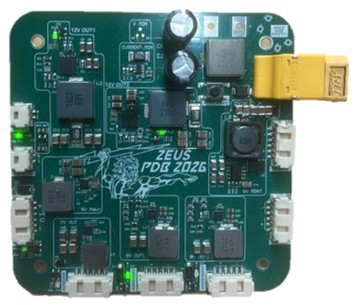
\includegraphics[width=0.7\textwidth,right]{pdb_board.jpg}

\end{minipage}
\end{figure}


\section{Description}
\begin{itemize}
    
\item  aaa
\end{itemize}
\newpage
\section{Technical specification}
\centering
\begin{tabular}{lcr}
\toprule
 & Unit & Value \\
\midrule
Input voltage& $V$ & 16.8/50.4\\
& & \\
& & \\
& & \\
& & \\
& & \\
& & \\
\bottomrule
\end{tabular}

\raggedright

\section{Pinout}

\centering
\begin{tabular}{lcr}
\toprule
  Pin & Signal \\
\midrule
1 &   \\
2 &   \\
3 &    \\
4 &   \\
5 &  \\
6 &   \\ 
\bottomrule
\end{tabular}



\raggedright
\section{Measures}
\centering
\begin{figure} [h]
\centering
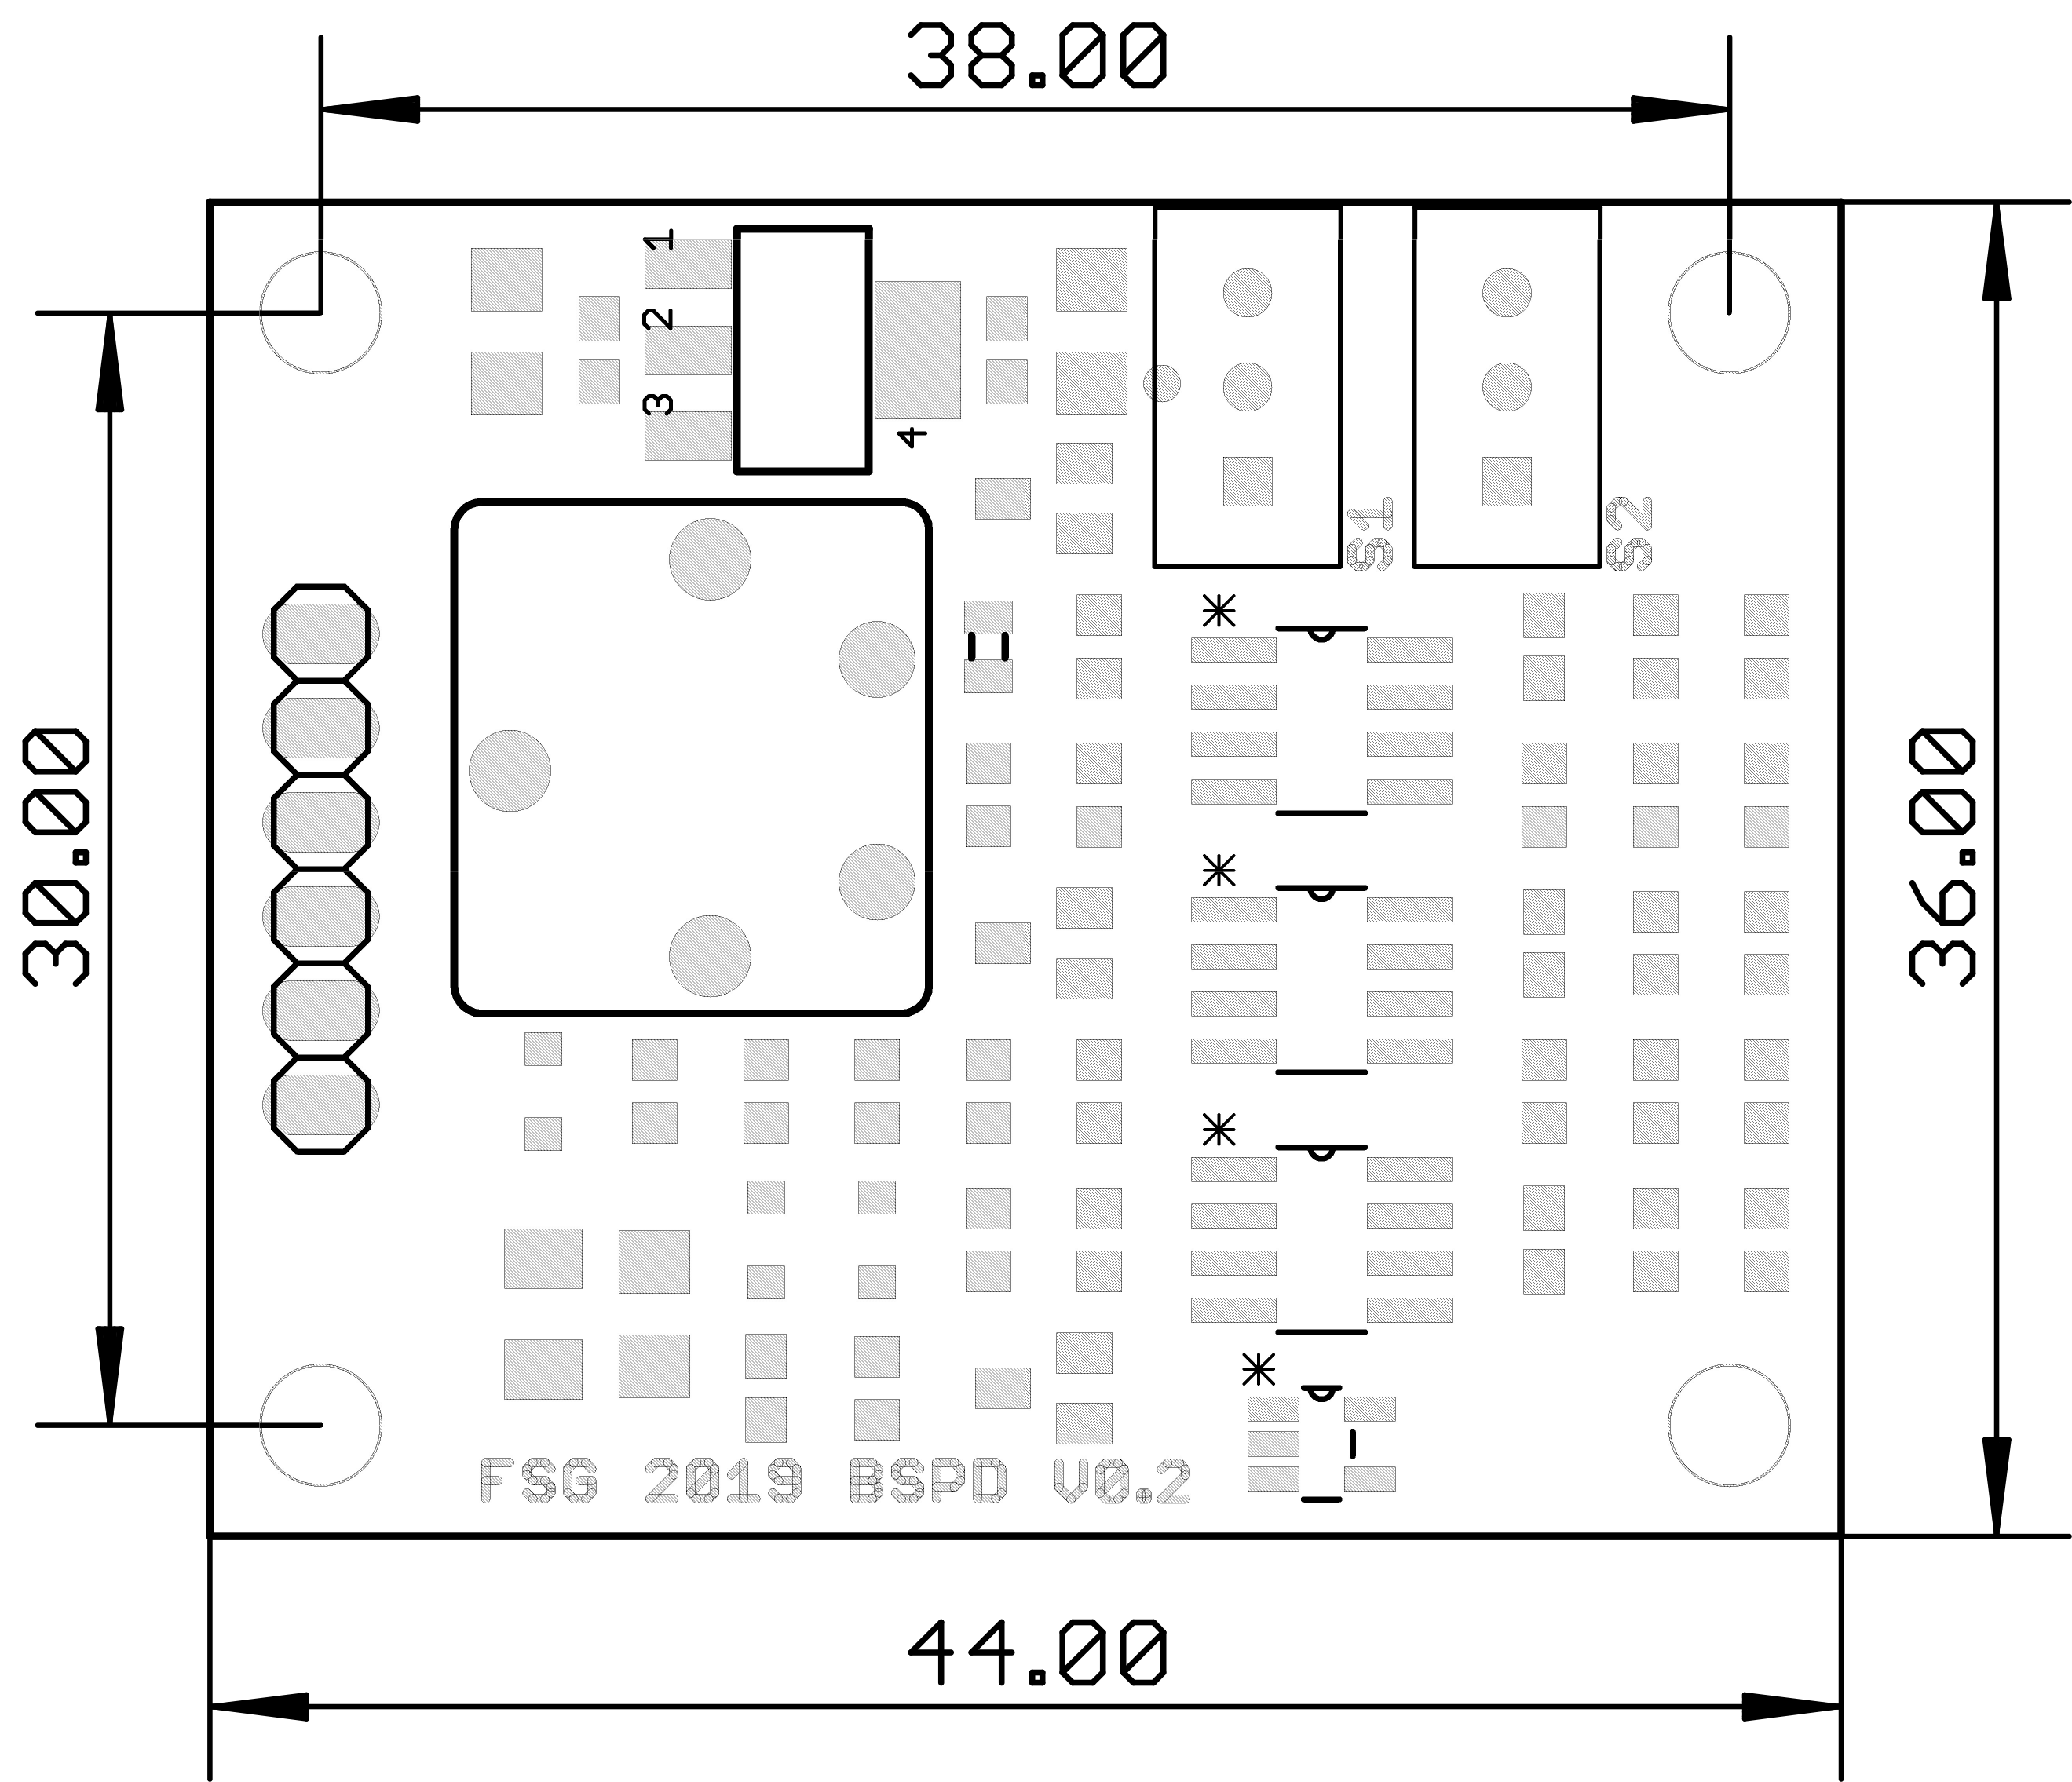
\includegraphics[width=0.7\textwidth,]{measures.png}

\end{figure}


\begin{figure}
\centering
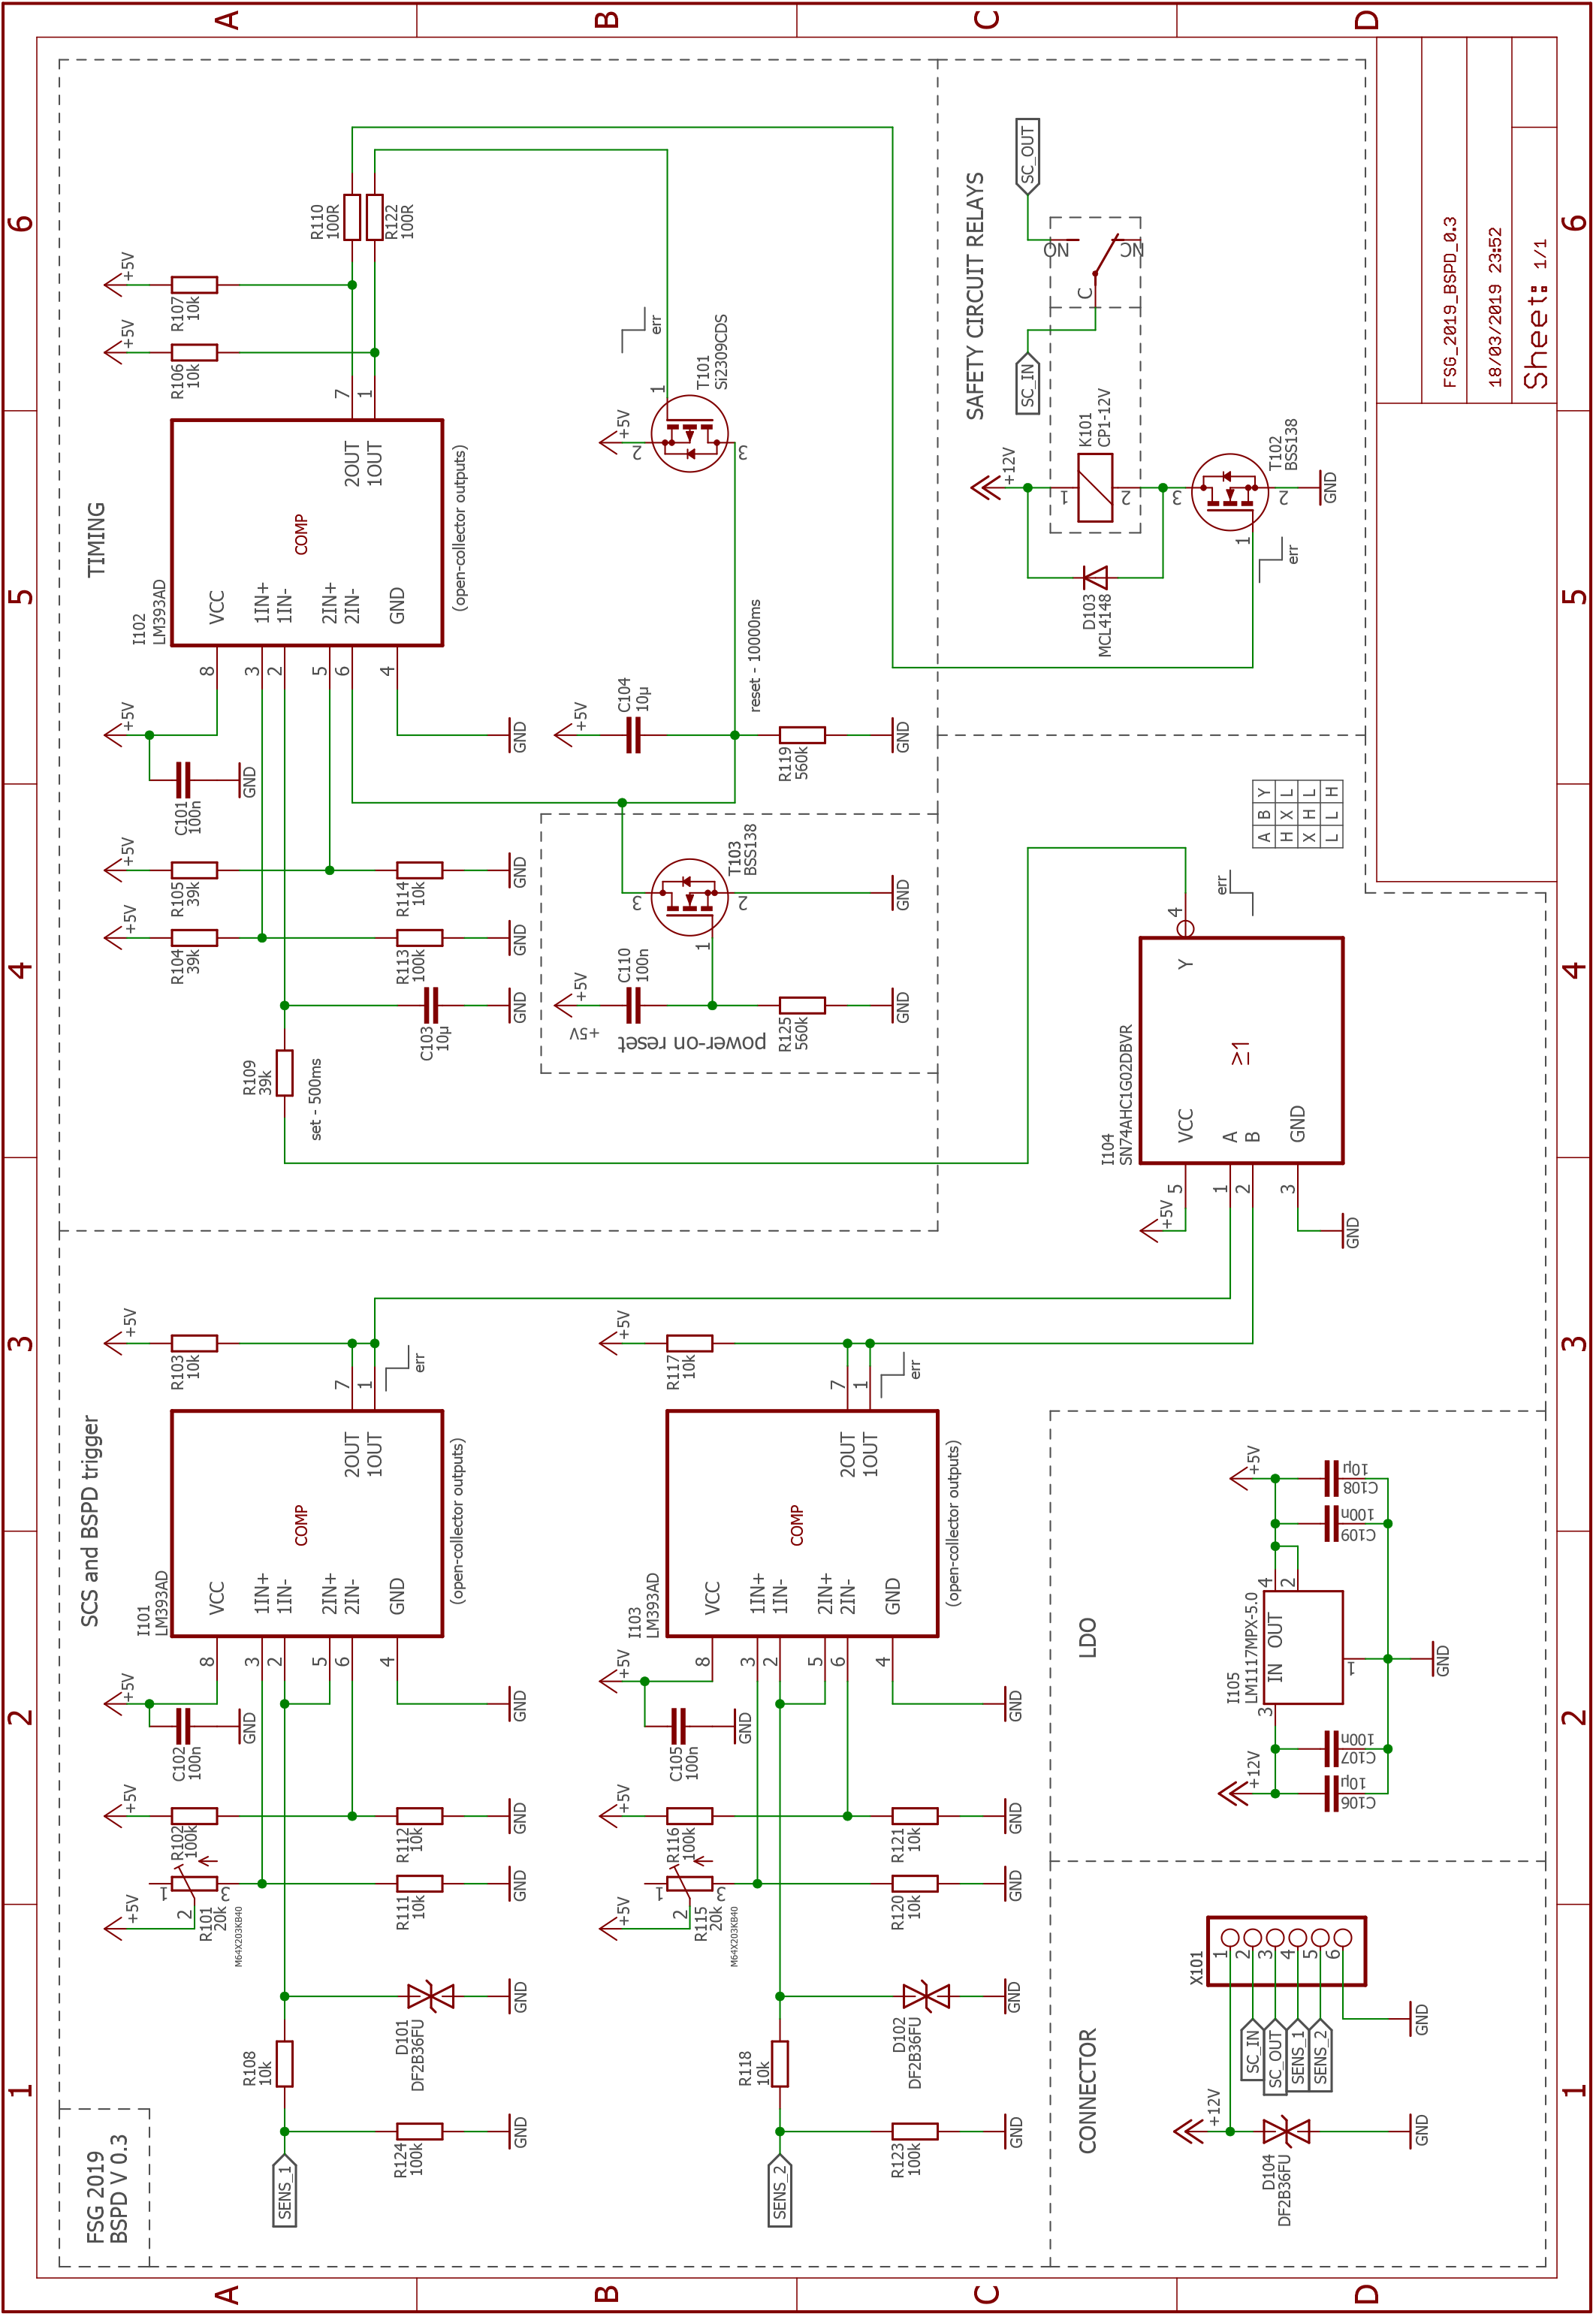
\includegraphics[width=1\textwidth,left,]{schematic.png}

\end{figure}

\begin{figure}
\centering
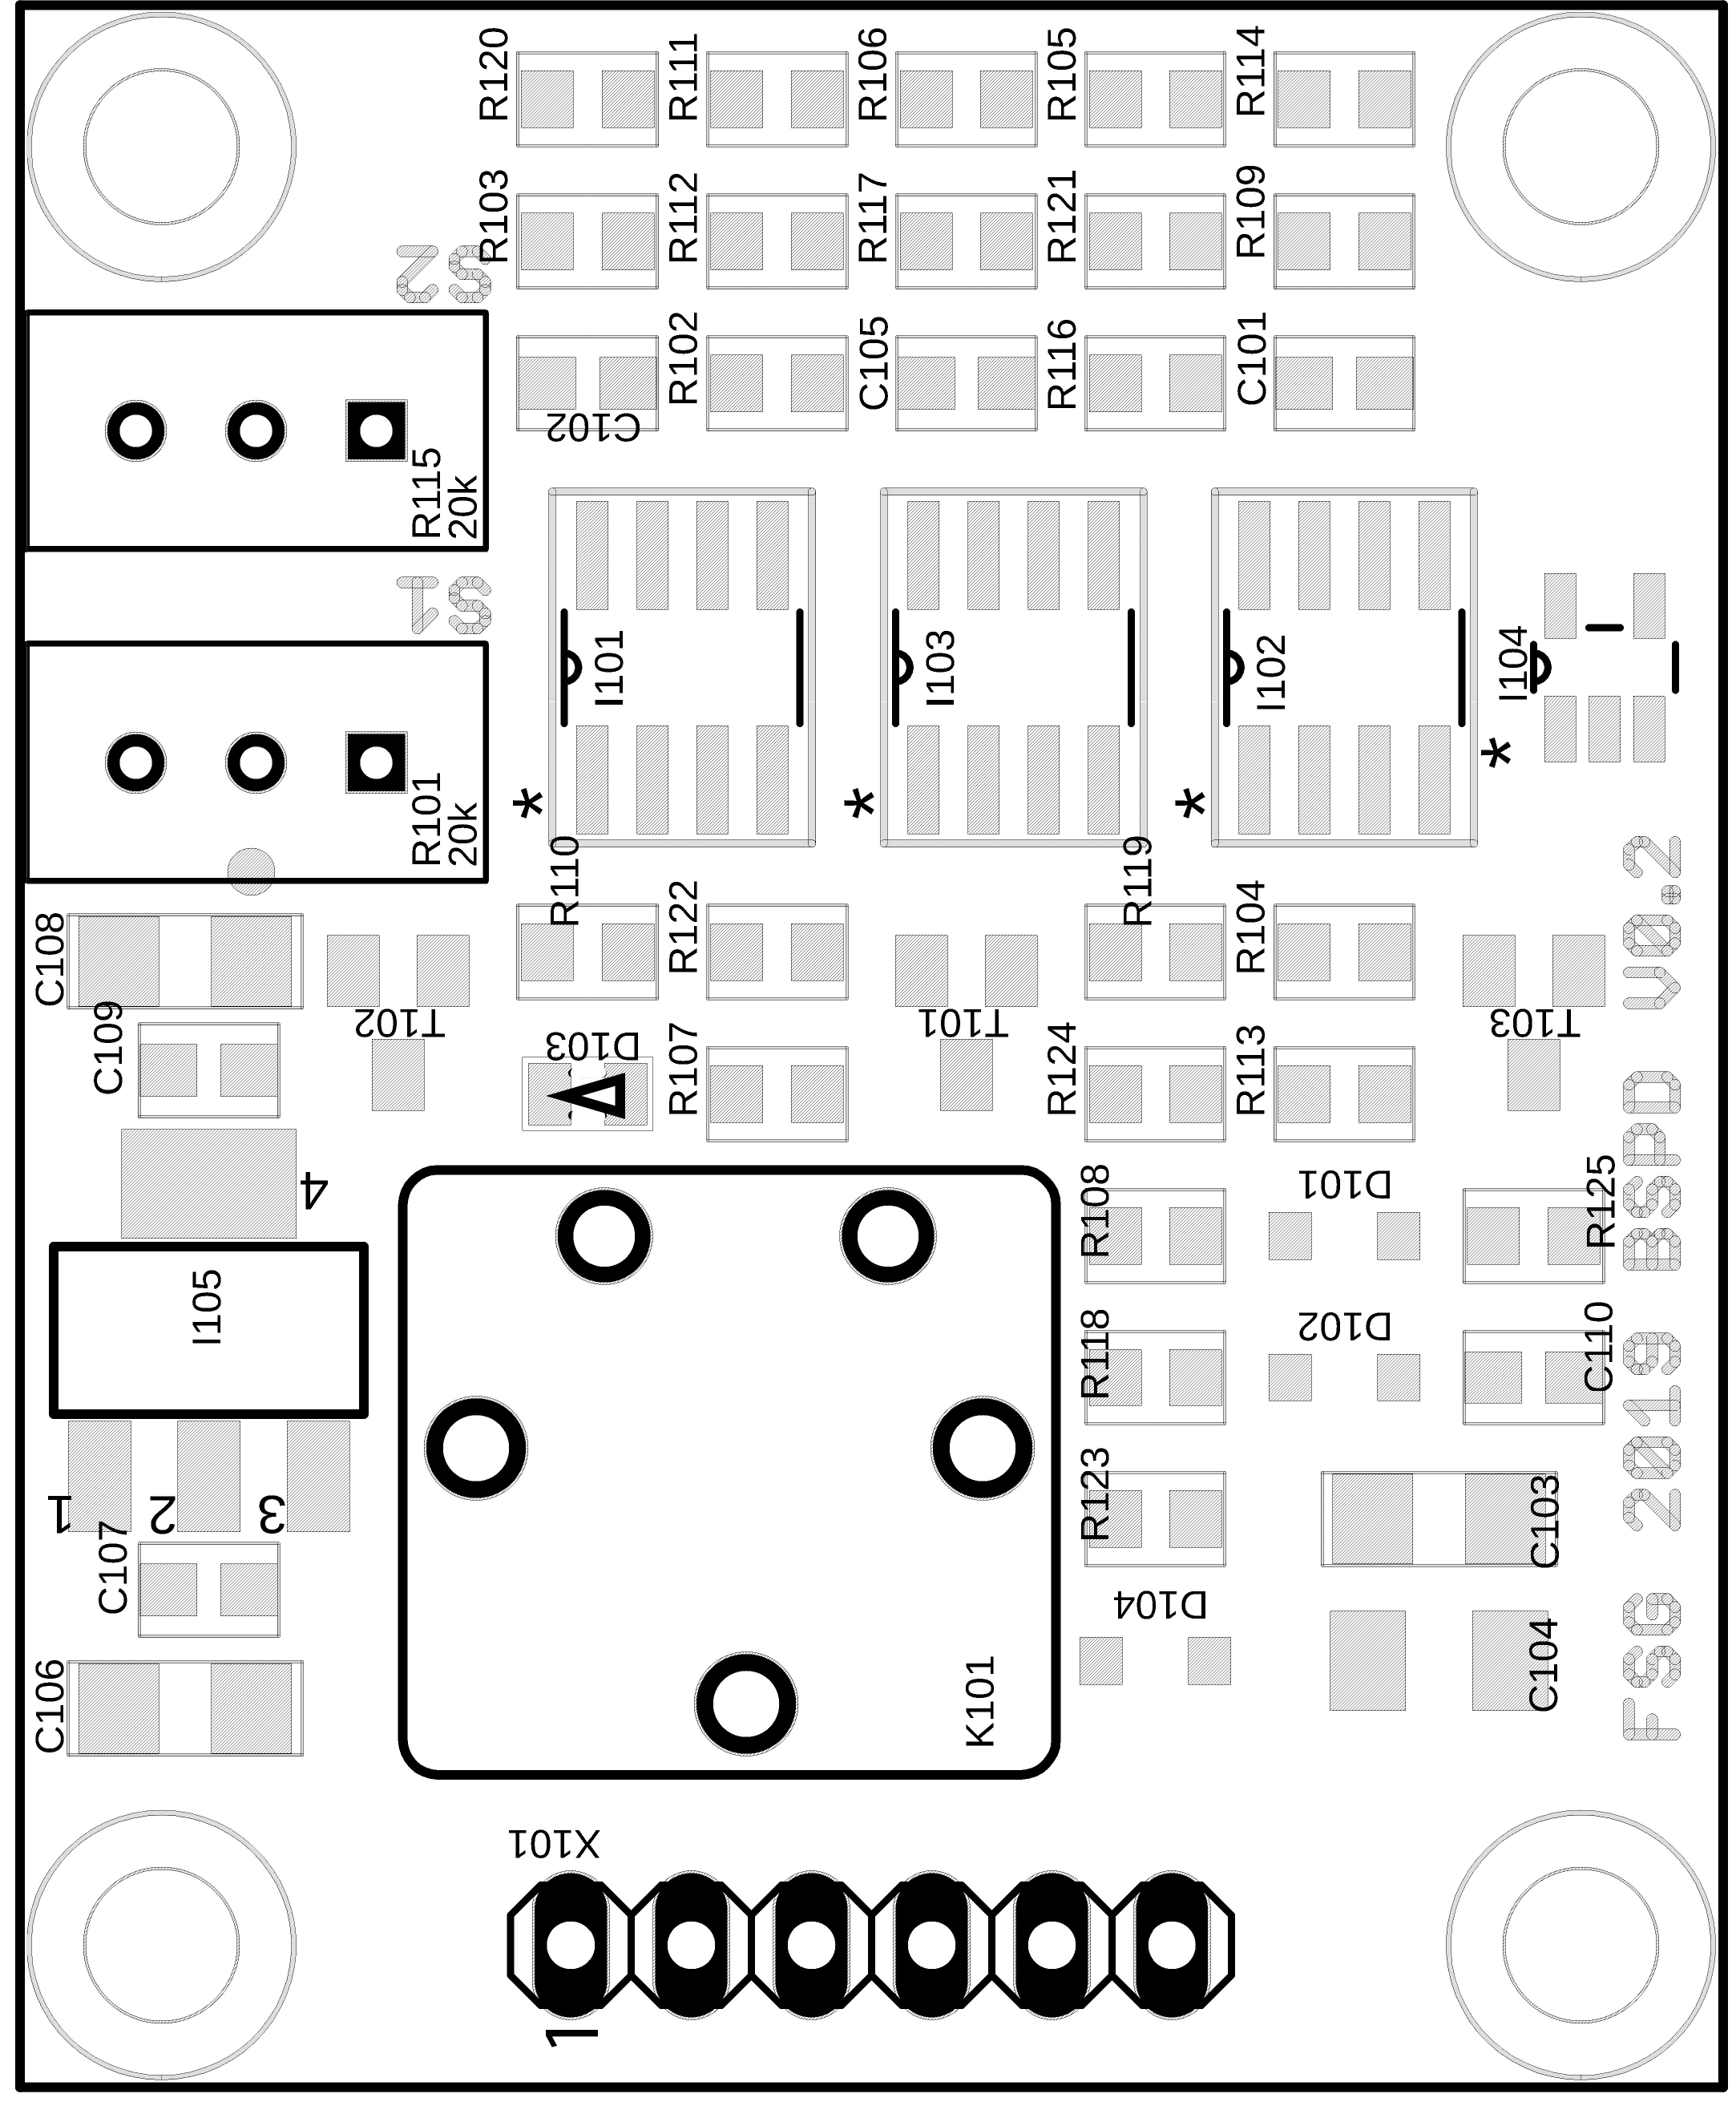
\includegraphics[width=1\textwidth,left,]{board.png}

\end{figure}
\end{document}



